\documentclass[11pt]{article}
\usepackage[english,magyar]{babel}
\usepackage{graphicx}
\usepackage{xcolor}
\usepackage[left=2.5cm, right=2.5cm]{geometry}
\usepackage{float}
\usepackage{hyperref}
\hypersetup{
	colorlinks=true,
	linkcolor=black,
	citecolor=black,
	filecolor=magenta,      
	urlcolor=cyan,
	pdftitle={WaveFunctionSimulation},
	pdfpagemode=FullScreen,
}
\usepackage[acronym]{glossaries}


\urlstyle{same}
\bibliographystyle{IEEEtran}

%-------------------------------------------------------
% Custom commands:

\newcommand\todo[1]{
\begin{LARGE}
	\textcolor{red}{TODO: #1}\\
\end{LARGE}
}

\newcommand{\probP}{\text{I\kern-0.15em P}}

%-------------------------------------------------------


\title{Time evolution simulation of the quantum mechanical wave function in 3D space}
\author{Zoltán Simon\\[1cm]{\small Advisors: Dr. Balázs Csébfalvi, Dr. Géza István Márk, Dr. Péter Vancsó}}

\makeglossaries
\newacronym{qm}{QM}{Quantum Mechanics}
\newacronym{gr}{GR}{General Relativity}
\newacronym{fft}{FFT}{Fast Fourier Transform}

\begin{document}
	\selectlanguage{english}
	
	\maketitle
	
	\begin{figure}[H]
		\centering
		\includegraphics[width=0.5\textwidth]{"figures/preview_image.jpeg"}
		\caption{Wave packet going through double-slit.}
		\label{fig:penetrating_potential}
	\end{figure}
	\thispagestyle{empty}
	\pagebreak
	\pagenumbering{arabic}
	
	\tableofcontents
	
	\pagebreak

	\section*{Abstract}
\selectlanguage{english}

In quantum mechanics, the wave function describes the state of a physical system. In the non-relativistic case, the time evolution of the wave function is described by the time-dependent Schrö\-din\-ger equation. In 1982, D Kosloff and R Kosloff proposed a method \cite{KOSLOFF198335} to solve the time-dependent Schrödinger equation efficiently using Fourier transformation.
%Injected part:
The computational physics research group, led by Géza I. Márk in the
Nanotechnology Departement, Institute for Technical Physics and
Materials Science, Centre for Energy Research, in collaboration with
Belgian researchers developed a simulation method based on
three-dimensional wave packet dynamics for the study of the electron
dynamics in nanosystems. A simplified, interactive two-dimensional
version for educational purposes was published in 2020 \cite{mark2020webschrodinger}. In this
work, we demonstrate two improvements of the wave packed dynamical
simulation software: (i) the use of \acrfull{gpu},
which results in a vast (up to 50x) increase in simulation speed, and (ii)
the introduction of advanced visualization techniques \cite{raytracing_weekend, csebfalvi2023} which
are important to correctly interpret huge 4D space-time wave function
data sets obtained from the simulation.
%End of injected part
%In 2020, Géza István Márk published a paper \cite{mark2020webschrodinger} describing a computer program for the interactive solution of the time-dependent and stationary two-dimensional (2D) Schrödinger equation. Some details of quantum phenomena are only observable by calculating with all three spatial dimensions. We found it worth stepping out from the two-dimensional plane and investigating these phenomena in three dimensions. We implemented the above method for the three-dimensional case to simulate the time evolution of the wave function.
We used our implementation to simulate typical quantum phenomena using wave packet dynamics. First, we tried the method on analytically describable cases, such as the simulation of the double-slit experiment, and then we investigated the operation of flash memory. We used raytraced volumetric visualization to render the resulting probability density. In our work, we introduce the basics of wave packet dynamics in quantum mechanics. We describe the used method in detail and showcase our simulation results.\\
For further information and animations, please visite\\ \url{https://zoltansimon.info/src/content/research/wavepacketsim.html}

%\selectlanguage{magyar}
%\section*{Kivonat}
%
%A kvantummechanikában a hullámfüggvény írja le egy fizikai rendszer állapotát. Nemrelativisztikus esetben a hullámfüggvény időbeli fejlődését az időfüggő Schrödinger-egyenlet határozza meg. 1982-ben D Kosloff és R Kosloff közölt egy módszert \cite{KOSLOFF198335} az időfüggő Schrödinger-egyenlet hatékony megoldására Fourier-transzformáció felhasználásával. 2020-ban Márk Géza István cikkében \cite{mark2020webschrodinger} bemutatott egy interaktív szá\-mí\-tó\-gé\-pes programot az időfüggő és a stacionárius kétdimenziós Schrödinger-egyenlet megoldására. A kvantumos jelenségek bizonyos részletei csak mindhárom térdimenzióval számolva figyelhetők meg. Érdemesnek tartottuk a síkból kilépve, térben is megvizsgálni ezeket a jelenségeket. Munkánkban háromdimenziós esetre implementáltuk az említett módszert, hogy szimuláljuk a hullámfüggvény időbeli fejlődését. Hullámcsomag-dinamikát használva kipróbáltuk több jellegzetes kvantumos jelenség szimulációját. A módszert először analitikusan kezelhető esetekre teszteltük, például a kétréses kísérlet szimulációjára, ezután megvizsgáltuk a flash memória cella működését. A szimuláció kimeneteként előálló valószínűségi sűrűséget sugárkövetéses térfogati megjelenítéssel ábrázoltuk. Dolgozatunkban ismertetjük a kvantummechanikai hullámcsomag-dinamika alapjait. Részletesen leírjuk a használt eljárást, és bemutatjuk a szimulációnk eredményeit.\\
%További információ és animációk találhatóak a\\ \url{https://zoltansimon.info/src/content/research/wavepacketsim.html} webcímen.
%
%\selectlanguage{english}


	\pagebreak
	
	\section{Introduction}

Quantum mechanics (QM) describes the behaviour of physical systems \cite{schwabl2007quantum}.
It is a common view that while Albert Einstein's General Relativity (GR) \cite{wald2010general} provides a model that accurately describes the laws of nature governing large scale phenomena, quantum theory is the best for small things.
Although humanity has not yet accepted a single theory that would be capable of modelling both the small and the large thus bridging the gap between QM and GR, there are many features of both mentioned theories that require effort to master.
In this writing we discuss a numeric approximation of the solution of one of QM-s fundamental equations,
the Schrödinger equation.
In non-relativistic QM the time dependent Schrödinger equation \cite{schrodinger1926} governs the time evolution of the wave function $\psi(\vec{r}; t)$, where $\vec{r}$ is the position vector and $t$ is the time.
This equation can be written in the form \ref{eq:schrodinger}.
\begin{equation}
	\label{eq:schrodinger}
	i\frac{\delta}{\delta{}t}\psi(\vec{r}; t) = H \psi(\vec{r}; t)
\end{equation}
Here $i$ is the complex unit, $\frac{\delta}{\delta{}t}$ is the partial differential operator with respect to time and $H$ is the $H$ is the Hamiltonian operator.
Consequently the properties of the physical system are encoded in the Hamiltonian.
If the potential is conservative, then $H = K + V$ is true, where $K$ is the kinetic energy operator and $V$ is the operator corresponding to the potential energy.
For local potentials the $V$ operation simply stands for a multiplication with the $V(\vec{r})$ position dependent potential value.
Generally solving equation~\ref{eq:schrodinger} analytically is not possible except for a few special cases such as the Hydrogen atom.

Géza I. Márk \cite{mark2020webschrodinger} presents a method to approximate the solution of the Schrödinger equation.
In his article he provides detailed description of separate methods for both the time dependent and the time independent equation's approximation.
In the focus of their article is an implementation called Web-Schrödinger.
This program is capable of approximating both the time dependent and the time independent equation for 2D spaces.
In our work we have only dealt with the time dependent version.
On the flip side, we implemented the method in 3D.






	
	\input{sections/our_method.tex}

	\section{Our implementation}
\label{sec:our_implementation}

Using the Fourier method we created a Python application simulating the time development of the quantum mechanical wave function.
We use ray tracing to visualize resulting volumetric of probability density.
The visualization requires the sampling of 3D data set on a discretized grid.
This makes it impossible to fully reconstruct the wave function that we simulated using only a finite resolution to begin with.
In order to fight sampling artifacts we deploy a state of the art triquadratic reconstruction filter recently proposed by Balázs Csébfalvi \cite{csebfalvi2023}.

We choose Python \cite{van1995python} as our programming language because there is a waste amount of helpful tools implemented to use with it that specifically aim towards leveraging the difficulty of writing mathematical and physics related simulation.
The majority of these tools are written in a hardware friendly languages such as Fortran, C or C++.
However they come with an easy-to-use \acrfull{api} that can be accessed from high level programming languages.
In these modern languages such as Python one works on a higher abstraction level usually not dealing with memory management ore pointer arithmetic.
Out implementation heavily depends on the Numpy library \cite{harris2020array}.
NumPy is a library that can be utilized to work efficiently with large arrays and tensors performing computationally intensive operations.
A similar library is SciPy \cite{2020SciPy-NMeth} also used in our program.
For 3D visualization we choose to use VisPy \cite{vispy}.
This library provides a nice basic set of features to handle virtual camera and create scenes but also enables us to go deeper and write our own \acrshort{gpu} shader code.
We made use of this to modify the default volume visualization code to fit our needs.

The Fourier method described in section \ref{sec:used_method} opens up the possibility to implement the simulation on the \acrshort{gpu}.
The \acrfull{cuda} toolkit is often used for parallel computational tasks implemented on the \acrshort{gpu} \cite{cuda2008}.
It comes with a powerful \acrshort{gpu} based \acrshort{fft} implementation.
To use \acrshort{cuda} with Python we selected the CuPy wrapping library \cite{cupy_learningsys2017} that provides abstraction over \acrshort{cuda}.
For other purposes we use multiple other libraries such as Imageio, Matplotlib, toml, Pillow, Keyboard, Colorama, Numba, Tqdm, PyQt5, PyOpenGL.
The sources for these libraries can be found on the internet.
We have listed the required versions in a requirements.txt file in the projects GitHub repository.

In its current state our application has only a console interface and it saves the resulting images and videos into files.
The reason that we so far haven't prioritized the development of a graphical user interface is that we think that terminal interfaces can still have their benefits even in 2023.
An application that only requires a terminal to function is simpler thus more effort can be made to improve the core functionality.
The audience of this software are scientists and engineers in the first place.
This is especially true in the early stage of development that we are currently in.
It already has however a snapshot system that makes it possible to interrupt a longer simulation and later resume from the exact state where it was previously halted.
This turned out to be a very convenient feature although since we use \acrshort{gpu} acceleration the simulation times are generally much shorter.
Our design philosophy dictated to communicate as much information about the simulated wave function towards the user as possible.
This direction can be thought of as controversial since too much data can obfuscate the important details especially in a plain console print.
We try to battle this effect by using colorful prints and by saving the text into a log file so that the parameters can be found even after the simulation has finished.

To specify the parameters of a simulation we use a configuration file in \acrfull{toml} format \cite{toml}.
The flexibility and universality of this data-format made it an overall good choice.
We can use a single \acrshort{toml} file to set the resolution and dimensions of the simulated volume, specify the parameters of the wave packet, add an arbitrary number of various potential barriers.
I this file we have parameters to configure the 3D visualization and others.

As we have mentioned earlier the output of the program gets saved in files.
The program creates images and videos and text files.
The images can be thought of as higher resolution snapshots from the videos but we also create images that are not corresponding to any of the videos.
Currently we generate five types of different images.
We call these canvas dwell time, canvas probability, per axis probability density, probability density 3D and finally, probability evolution.
In each of these categories a sequence of images is being generated for each run of the simulation.
The interval at which the state of the simulation is captured can be specified in the above described configuration file.
Canvas dwell time is the integral of probability density over time in a specified plane intersecting the simulated volume.
Canvas probability is the probability density in a specified plane intersecting the volume.
Both dwell time and probability density can be used to visualize interference patterns after a wave packet passes through some kind of a potential barrier such as a double-slit or an optical grid.
Per axis probability density gives a projected view on the probability density.
This not a real image but rather a plot of probability density as the function of spatial coordinates separately for each axis.
To obtain this plot we integrated the probability density so that for a specific $i_j = x$ discretized spatial coordinate we sum the probability density where $i_j = x$ and the other two coordinates run across their domain.
We also overlap the plot of the potential barriers on the same graph.
This helps to understand the changes in propagation of the wave packet.
This type of plot can provide useful information for most of the simulation cases, but it is especially useful when we want to simulate the behavior of three one dimensional particles in a three dimensional configuration space.
In this case the projected probability density along each axis represent the wave packet of a different 1D particle.
It is possible to initialize a potential that model the collision between these three particles.
This creates the effect that the particles interact.
In the configuration file there is a possibility to set whether a potential barrier should appear in the visualization.
By disabling the visualization of the interaction potential we can get rid of any hardly conceptualizable elements of the resulting potential and maybe focus on a wall or a harmonic oscillator instead.
Probability density 3D is the most self explanatory output of the system.
Here we take the probability density as a 3D volumetric data set and visualize it using ray tracing.
Ray tracing is the method where 





	\section{Results}
\label{sec:results}

\subsection{General approach and the system of units}

We used our software to perform various \acrshort{wpd} simulations.
In this section, we present the results of some of these simulations.
We will shortly introduce the simulated scenarios.
We also want to provide some formulas to validate the correctness of some of the simpler scenarios analytically.
Our simulator uses the Hartree atomic units \cite{hartree_1928}.
Every quantity in the upcoming part should be interpreted as such.
This unit system makes it convenient to deal with quantities at atomic scale.
You can find animations showing the time evolution of \acrshort{wp}s simulated by our software on  \url{https://zoltansimon.info/src/content/research/wavepacketsim.html}.
From this web page, you can also navigate to the GitHub repository of our project, where all our source code is available for download.

\subsection{Double-slit experiment}

First, we would like to present the simulation results of an electron scattering experiment.
Scattering of a particle happens when the \acrshort{wp} of the particle passes through some kind of a barrier with holes in it.
In our simulation, we can model the barrier as a localized potential.
The \acrshort{wp} arrives from one side of the barrier.
While passing through this barrier, it scatters, and some of the \acrshort{wp} gets reflected back.
The portion of the \acrshort{wp} that passed through --suffering scattering-- continues forward and consequently arrives at a measuring device\footnote{In scattering and diffraction experiments we can make the distinction between a near field and far field solution.}.
In our simulation, our measuring device is a virtual canvas where we measure the probability density.
A simple scattering scenario is the double-slit experiment.
Here the barrier is a potential wall with two narrow parallel slits.
The \acrshort{wp} passes through these slits.
According to the Huygens–Fresnel principle in scattering experiments, we can approximate the wave function after the barrier as concentric waves emitted from the slits or holes of the barrier.
This gives a simple enough model to predict the shape of the interference pattern forming on the canvas.
We would like to validate the distance between the stripes in the interference pattern.
To calculate the distance between the probability density peaks, first, we have to get a formula for the intensity on the canvas.
\begin{equation}
	\label{eq:Huygens}
	I(\vec{r}) = I_0 \frac{sin^2\left( \pi N \frac{dy}{\lambda L} \right)}{sin^2\left( \pi \frac{dy}{\lambda L} \right)}
\end{equation}
where $N$ is the number of holes on the barrier (in double-slit experiment $2$), $d$ is the distance between the center of the holes, $L$ is the distance between the canvas and the barrier $\lambda$ is the wavelength of the wave and $y$ is the location on the canvas.
We performed the simulation using $L = 30$ Bohr radii, $d = 4.0$ Bohr radii, $\lambda = \frac{2\pi}{3}\simeq 2.1$ Bohr radii with two slits.
The width of each slit was a small enough value of $1.0$ Bohr radii.
\begin{figure}[hbt!]
	\begin{center}
		\includegraphics[width=0.45\textwidth]{figures/double_slit_01.png}
		\includegraphics[width=0.45\textwidth]{figures/double_slit_02.png}
		\includegraphics[width=0.45\textwidth]{figures/double_slit_03.png}
		\caption{Stages of the double-slit experiment: before, during, and after passing through the double-slit}
		\label{fig:double_slit_stages}
	\end{center}
\end{figure}
Different stages of double-slit simulation can be seen in figure \ref{fig:double_slit_stages}, where we have used ray tracing to visualize the probability density and the potential.
The interference pattern is visualized in figure \ref{fig:double_slit_interference} on a canvas of size $60 \times 60$ Bohr radius.
We compared the simulated pattern and the pattern predicted by the Huygens–Fresnel principle.
It can be seen that the two patterns are very similar.
The animation of this simulation can be accessed on \url{https://www.youtube.com/watch?v=16M21MPFea0}.
\begin{figure}[hbt!]
	\begin{center}
		\includegraphics[width=0.6\textwidth]{figures/double_slit_interference.png}
		\includegraphics[width=0.6\textwidth]{figures/validation_of_double_slit.png}
		\caption{Comparison of the simulated (above) and the analytically predicted (below) interference pattern during double-slit experiment}
		\label{fig:double_slit_interference}
	\end{center}
\end{figure}

\subsection{Diffraction by optical grating-like potential}

Many different forms of diffraction can be explained using \acrshort{qm}.
The scale at which diffraction happens ranges from the scale of subatomic particles to larger molecules.
Measuring diffraction patterns is a handy tool in the hands of scientists.
It provides information about the object that caused the diffraction.
At this point, it is essential to emphasize that the diffraction of light is a different phenomenon from the diffraction of matter waves since light is an electromagnetic wave.
With that said, the fact that particles are not electromagnetic waves but still exhibit wave-like behavior, as discussed in Section \ref{sec:theory} makes this experiment even more interesting.
Note that in equation \ref{eq:Huygens}, the $y$ is a one-dimensional coordinate. Indeed, the double-slit experiment can be fully described using only two spatial dimensions, and the diffraction pattern forms in a single dimension perpendicular to the propagation direction of the wave.
This is because the localized potential in this scenario is independent of the $z$ coordinate.
To make use of all three simulated dimensions, we also modeled diffraction on diffraction gratings.
In optics, a diffraction grating is a periodic 2D structure that diffracts light \cite{Stroke1967}.
In \acrshort{qm}, such gratings can also be utilized to diffract wave packets.
The holes between the potential nodes behave like the holes in the double-slit experiment.
We put 11 nodes in each direction, forming a rectangular grid.
We experimented with various lattice constants (distance between adjacent grid points).
Here, we present two simulations.
In the first simulation, each node has a Gaussian potential distribution and a maximal potential of $V_{max} = 8$ hartree.
The distance between adjacent grid points is $d = 4$ Bohr radii.
In the second simulation, each node has a Gaussian potential distribution and a maximal potential of $V_{max} = 25$ hartree.
The distance between adjacent grid points is $d = 8$ Bohr radii.
The canvas distance is $L=30$ Bohr radii, and the wavelength of the \acrshort{wp} is $\lambda\simeq 2.1$ Bohr radii for both simulations.
Note in both cases the kinetic energy of the \acrshort{wp} $E = \frac{p^2}{2m} = \frac{h^2}{2\lambda^2} \simeq 4.5$ hartree is less than $V_{max}$.
Otherwise, the grating would not impact the propagation of the \acrshort{wp} sufficiently.
In figure \ref{fig:optical_grid_stages}, we visualized different stages of the time development of the first simulation, and \ref{fig:optical_grid_stages_8_bohr_radii} showcases stages of the second simulation.
Both sequences of rendered images make use of the ray tracing visualization method.
\begin{figure}[hbt!]
	\begin{center}
		\includegraphics[width=0.45\textwidth]{figures/optical_grid_01.png}
		\includegraphics[width=0.45\textwidth]{figures/optical_grid_02.png}
		\includegraphics[width=0.45\textwidth]{figures/optical_grid_03.png}
		\caption{Stages of the diffraction grating experiment using a grating with lattice constants of $4$ Bohr radii: during, right after, and later after passing through the grating}
		\label{fig:optical_grid_stages}
	\end{center}	
\end{figure}
\begin{figure}[hbt!]
	\begin{center}
		\includegraphics[width=0.45\textwidth]{figures/optical_grid_8_bohr_rad_01.png}
		\includegraphics[width=0.45\textwidth]{figures/optical_grid_8_bohr_rad_02.png}
		\includegraphics[width=0.45\textwidth]{figures/optical_grid_8_bohr_rad_03.png}
		\caption{Stages of the diffraction grating experiment using a grating with lattice constants of $8$ Bohr radii: during, right after, and later after passing through the grating}
		\label{fig:optical_grid_stages_8_bohr_radii}
	\end{center}	
\end{figure}

During the simulation, many interesting interference patterns arise.
We showcase some of these for the $4$ Bohr radius lattice constant case in figure \ref{fig:optical_grid_interference} and for the $8$ Bohr radius lattice constant case in figure \ref{fig:optical_grid_interference_8_grid}.
The animations showing the results in motion can be found on \url{https://youtu.be/KCE5xqm-diQ?si=-kzjWvaw8zOcAz4C} and \url{https://youtu.be/YCadOpsx9y8}.
\begin{figure}[hbt!]
	\begin{center}
		\includegraphics[width=0.49\textwidth]{figures/optical_grid_interference_01.png}
		\includegraphics[width=0.49\textwidth]{figures/optical_grid_interference_02.png}
		\caption{Two stages of interference patterns forming on the measurement canvas during diffraction grating simulation using lattice constant of $4$ Bohr radii}
		\label{fig:optical_grid_interference}
	\end{center}	
\end{figure}
\begin{figure}[hbt!]
	\begin{center}
		\includegraphics[width=0.49\textwidth]{figures/optical_grid_interference_01_8_grid.png}
		\includegraphics[width=0.49\textwidth]{figures/optical_grid_interference_02_8_grid.png}
		\caption{Two stages of interference patterns forming on the measurement canvas during diffraction grating simulation using lattice constant of $8$ Bohr radii}
		\label{fig:optical_grid_interference_8_grid}
	\end{center}	
\end{figure}

\subsection{Many-body interactions}

One interesting use case of a higher dimensional \acrshort{wpd} simulator is that the higher dimensional space can be used to model the interactions between multiple lower-dimensional particles.
For example, our 3D simulation is capable of the simulation of three 1D particles.
To do this, we have to define special interaction potential.
To create such potential, we have to think about the coordinates in the higher dimensional configuration space as the coordinates of the lower dimensional space describing the location of the lower dimensional particle.
If the potential energy affecting all particles can be expressed as a $V(x_a, x_b, x_c)$ function of the location of particle $A$ and $B$ and $C$, then we can reinterpret this function as the $V(\vec{r})$ localized potential function used in the potential propagator in equation \ref{eq:potential_prop}.
Note that here $\vec{r}$ becomes $(x_a, x_b, x_c)$.
To model the interaction between the three 1D particles, we initialized a linear combination of two types of interaction potentials.
One is proportional to $\frac{1}{|x_i - x_j|}$ where $i,j\in\{a,b,c\}$ and $i\neq j$ and the other is a hard interaction that takes its maximum if the particles approach each other inside an $\epsilon$ radius otherwise it is zero.
To prevent blotting of the Gaussian \acrshort{wp} we also initialized a harmonic oscillator potential.
This helps because the Gaussian \acrshort{wp} is the eigenstate of the harmonic oscillator.
The potential for a harmonic oscillator is given in the following form
\begin{equation}
	\label{eq:harmonic_osc}
	V(x) = \frac{m\omega^2}{2}x^2
\end{equation}
where $m$ is the oscillating mass and $\omega$ is the angular frequency of the oscillation.
Our first simulation of 1D particles is somewhat similar to the classical Newton's cradle \cite{Gauld2006}
in the sense that it demonstrates momentum transfer between multiple particles.
We created a scenario where particle $A$ starts at $25$ Bohr radii away from the center of the oscillator where the potential energy is maximal; thus, it accelerates towards the other two particles ($B$ and $C$), consequently transferring the momentum to particle $C$ on the far right.
For this experiment, the interaction potential consists only of the hard interaction.
The angular frequency of the oscillator was selected to be $\omega = \frac{2\pi}{40} \simeq 0.1571\; \frac{rad\cdot hartree}{\hbar}$.
After the momentum transfer, particle $C$ propagates towards the maximal potential of the oscillator on the far right.
Particle $B$ stays in place since it serves only as a medium in the momentum transfer.
The momentum gained from particle $A$ was immediately given to particle $C$.
When all the kinetic energy of the moving particle is transferred to potential energy, then it turns back.
The oscillation with the momentum transfer between the particles continues.
Different phases of this simulation can be observed on the per-axis visualization in figure \ref{fig:1d_particles_in_oscillator_stages}.
The corresponding animation can be found on \url{https://youtu.be/zOiYACVOssU}.
\begin{figure}[hbt!]
	\begin{center}
		\includegraphics[width=0.45\textwidth]{figures/1d_oscillator_01.png}
		\includegraphics[width=0.45\textwidth]{figures/1d_oscillator_02.png}
		\includegraphics[width=0.45\textwidth]{figures/1d_oscillator_03.png}
		\caption{Stages of the interactions between 1D particles in harmonic oscillator: initial state, particle A giving momentum to particle C, particle C reaching maximal potential and turning back}
		\label{fig:1d_particles_in_oscillator_stages}
	\end{center}
\end{figure}
Please note that particle $C$ converts all of its kinetic energy to potential energy right at the half of the first period of the oscillation $t = 40 / 2 \frac{\hbar}{hartree} = 20 \frac{\hbar}{hartree}$.
This means that the harmonic oscillator functions correctly.

Now, let us repeat this experiment, but now we place a finite potential barrier in the middle of the oscillator.
In Tamás Geszti's book \cite{geszti2007}, we can find that the probability of a particle with $E$ energy tunneling through a $d$ thick barrier of $V_0$ potential can be expressed in the following form
\begin{equation}
	\label{eq:tunneling_probability}
	\probP_{tunnel} = \frac{1}{1 + \frac{V_0^2}{4E(V_0 - E)}sinh^2(\kappa d)}
\end{equation}
where $\kappa = \sqrt{2m(V_0 - E)}\;/\hbar$ is determined by the energy of the incoming \acrshort{wp}.
Energy is conserved, so $E = V(x_A)$.
We solve for $\probP_{tunnel} = \frac{1}{2}$.
One possible solution is $V_0 \simeq 9.8$ hartree and $d \simeq 0.3$ Bohr radius.
Particle $A$ gives its momentum to $B$ as before.
With these parameters, approximately half of the probability density of particle $B$ tunnels through the barrier, giving its momentum to particle $B$ on the next side of the wall.
This causes the $C$ to start moving with a probability of approximately $\frac{1}{2}$.
What we just described is called the entanglement of the states of particles $A$, $B$, and $C$.
Let's perform a measurement to determine the location of particles $A$, $B$, and $C$ shortly after the first momentum transfer could have happened.
If we would measure particle $A$ to be located in the middle of the harmonic oscillator, that means that it gave its momentum to particle $B$ and $B$ has tunneled through the finite potential barrier.
If $B$ tunneled, that also means that beyond the barrier, it collided with particle $C$, consequently transferring all its kinetic energy to $C$.
On the contrary, if the result of the measurement determining the location of particle $A$ would have shown that particle $A$ bounced back from $B$, that means that $B$ did not tunnel through the barrier.
This also means that particle $C$ did not receive any kinetic energy and stayed stationary right beyond the barrier.
The measurement of the state of one entangled particle determines the outcome of the measurement of the other entangled particles.
Real-life experiments are sound with this thought experiment \cite{Vasilyev2017}.
The probability density plot can be observed in figure \ref{fig:1d_osc_with_tunneling}.
The animation of this simulation can be found on \url{https://youtu.be/IVb_mpzmuYA}.
\begin{figure}[hbt!]
	\begin{center}
		\includegraphics[width=0.45\textwidth]{figures/1d_oscillator_tunneling_01.png}
		\includegraphics[width=0.45\textwidth]{figures/1d_oscillator_tunneling_02.png}
		\includegraphics[width=0.45\textwidth]{figures/1d_oscillator_tunneling_03.png}
		\caption{Stages of the interactions between 1D particles in harmonic oscillator with finite potential barrier: initial state, particle A giving momentum to particle C with approximately 0.5 probability, particle C reaching maximal potential and turning back with approximately 0.5 probability}
		\label{fig:1d_osc_with_tunneling}
	\end{center}	
\end{figure}

\subsection{Modeling a flash memory cell}

Our last group of simulations tries to model the working of a flash memory cell.
Flash memory is used extensively in many modern electronic devices such as smartphones, laptops, or tablets.
The general structure of a cell is visualized in figure \ref{fig:flash_memory}.
The structure of a flash memory cell resembles a \acrfull{mosfet} \cite{Korec2011}.
The difference is that the memory cell has two gates: the control gate, which is connected to a control line similarly to regular transistors, and the floating gate, which is insulated from all sides by oxide layers.
Both the control gate and the floating gate are made out of conducting material (metal or polysilicon).
In figure \ref{fig:flash_memory}, it can be seen that between the control gate and the floating gate, there is a thicker potential barrier.
This prevents the flow of electrons between these two parts.
Only the Coulomb potential induced by the electrons on the control gate must be felt by the electrons on the floating gate.
A flash memory cell stores information by trapping electrons on a floating gate.
The reading of a memory cell is done by inducing a current through the channel between the source and drain.
If there are electrons trapped on the floating gate, they create an electric field affecting the substrate.
The substrate is made out of semiconducting material. (Generally silicon.)
A semiconductor changes conductivity based on the electromagnetic field.
If there are electrons on the floating gate, the channel between the source and drain has higher resistance.
By measuring the current through this channel, the information about the state of the floating gate can be retrieved.
This is used to store bits of information.
In our model, we simulate one single cell, and this cell only stores a single bit of information.
We only model one single electron that can be trapped on the floating gate.
The writing and flushing of the flash cell are performed by applying voltage on the control gate, inducing a strong enough electric field that the electron can tunnel through the potential barrier between the floating gate and the channel.
\begin{figure}[hbt!]
	\centering
	\includegraphics[width=0.5\textwidth]{figures/flash_memory.pdf}
	\caption{Schematic structure of a flash memory cell}
	\label{fig:flash_memory}
\end{figure}
For the writing and flushing to be possible, the thickness and height of the oxide layer --consequently, the potential wall-- between the floating gate and the substrate must be chosen carefully.
This barrier must be thick enough to prevent unwanted tunneling when no voltage is applied to the control gate.
After the control gate fills with electrons, the Coulomb potential created by those electrons makes an overall slope in the potential barrier created by the oxide layer.
The potential level inside the floating gate does not acquire a slope since it is made out of conducting material, hence its equipotential.
This slope is added to the potential barrier, thus changing its shape.
The previously rectangular barrier now acquired a triangular outline. More importantly, the $d$ width of the barrier gets reduced.
This increases the probability of the electron in the floating gate tunneling out from the gate through the thin oxide layer into the substrate.
This phenomenon is called Fowler–Nordheim tunneling \cite{Fowler_1928bv}.
Figure \ref{fig:fowler_nordheim_tunneling} visualizes the principle of this effect.
\begin{figure}[hbt!]
	\centering
	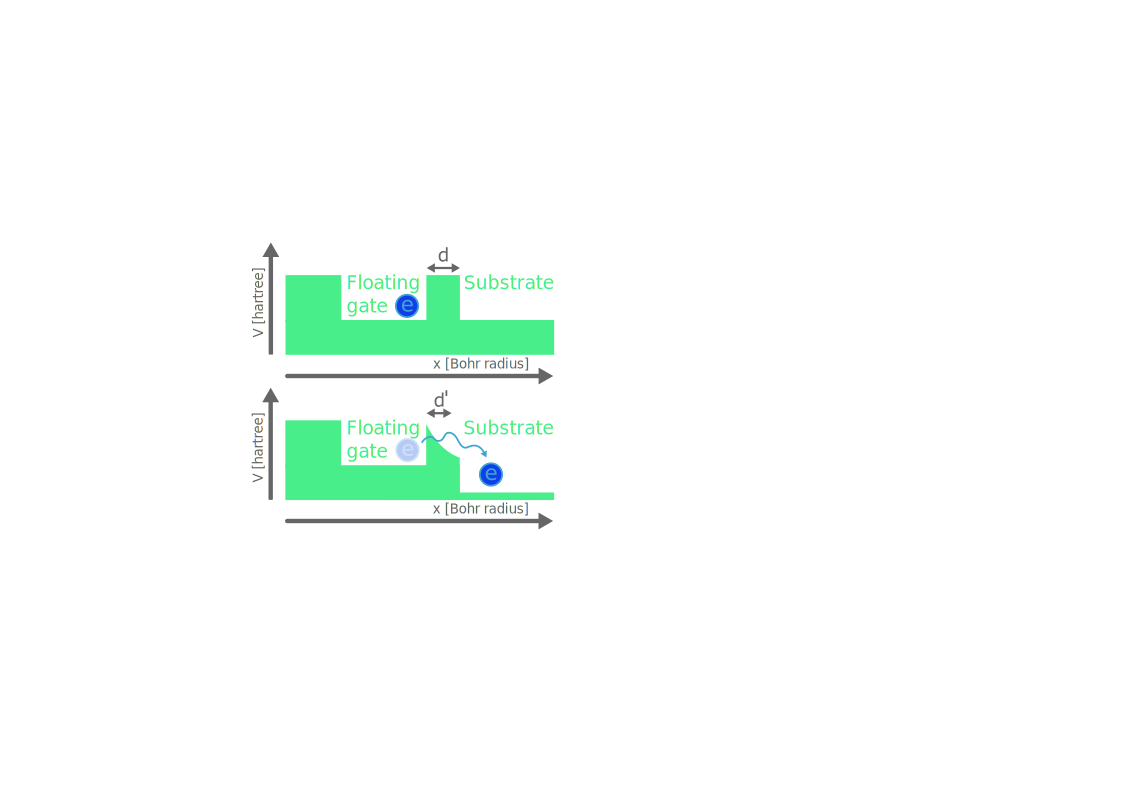
\includegraphics[width=0.5\textwidth]{figures/fowler_nordheim_tunneling.pdf}
	\caption{Fowler-Nordheim tunneling: on the upper image there is no Coulomb potential; on the image below Coulomb potential changes the shape of potential barrier causing tunneling}
	\label{fig:fowler_nordheim_tunneling}
\end{figure}
In our flash memory cell simulation, we initialized a potential wall representing the barrier between the floating gate and the substrate.
Our simulation deals with only one electron.
To simulate the flushing of the gate, we initialize the location of this electron to be inside the floating gate.
We add a Coulomb potential that decreases inside the thin oxide layer towards the substrate.
We initialized the barrier with a height of $V_0 = 10$ hartree and width of $d = 4.0$ Bohr radius.
We surrounded the floating gate area with thick potential barriers from the remaining five sides to prevent tunneling in unwanted directions. However, we excluded these from the visualization to make the electron's probability density visible from the outside.
We model the charge on the control gate as a uniformly charged infinite sheet.
This way, the Coulomb potential induced by a negatively charged control gate acting on an electron inside the oxide can be described by the following formula
\begin{equation}
	\label{eq:coulomb_potential}
	V_C = \frac{\sigma}{2r\epsilon}
\end{equation}
where $\epsilon$ is the dielectric permittivity of the oxide, $\sigma$ is the surface charge density at the control gate, and $r$ is the distance from the control gate.
Inside the floating gate, the potential stays zero.
On the thin oxide layer between the floating gate and the substrate, the slope of the potential has to be significant enough so that the probability of tunneling increases.
We initialized the Coulomb potential to create a steep enough slope at the start of the oxide.
For this, we set the charge density to $600 \frac{elementary charge}{(Bohr radius)^2}$ and the thickness of the oxide between the control gate and the floating gate to $10$ Bohr radius.
This is significant because although the gate is on equipotential, right after the gate, the Coulomb potential continues to decrease.
For simplicity, we choose $\epsilon$ to be equal to one.
With this setup the derivative of potential at the start of the oxide is $V' = \frac{d}{dr}\frac{\sigma}{2r\epsilon} = -\frac{\sigma}{2r^2\epsilon} = -\frac{600}{2\cdot 10^2\cdot 1} = 3\; \frac{\text{hartree}}{\text{Bohr radius}}$.
The potential barrier between the floating gate and the substrate was chosen to be $1$ Bohr radius thick and $8$ hartree high.
An electron inside the floating gate would have some kinetic energy, so we gave it an initial momentum of $3\; \frac{\hbar}{\text{Bohr radius}}$.
We ran the simulation with the Coulomb potential turned on and off and compared the \textit{probability evolution} plots.
Figure \ref{fig:flash_flush_plot} shows the flushing of the floating gate with the Coulomb potential enabled.
The probability of the electron being found on the floating gate is decreasing.
The step-like nature of the plot is caused by the bouncing of the wave packet inside the gate.
Also, note that the probability of the particle being found inside full volume is decreasing.
This is because we left the underside of the substrate open to prevent unwanted reflections from that barrier.
In that direction, the tunneling particle can leave the substrate freely.
In our simulation, the parts of the \acrshort{wp} leaving the visualized area get absorbed by the draining potential.
At first glance, the rate at which the particle leaves the gate seems slow.
Bear in mind that we are working with atomic units.
Figure \ref{fig:flash_flush_plot} shows that after $40\;\frac{\hbar}{\text{hartree}} \simeq 0.96 \text{femtoseconds}$ the probability of the particle located on the gate decreased by $10\%$.
\begin{figure}[hbt!]
	\centering
	\includegraphics[width=0.5\textwidth]{figures/flash_flush.png}
	\caption{Flushing of the floating gate: the probability of the particle being found on the floating gate is gradually decreasing}
	\label{fig:flash_flush_plot}
\end{figure}
In figure \ref{fig:flash_keep}, however, the electron stays on the gate since we disabled the Coulomb potential.
\begin{figure}[hbt!]
	\centering
	\includegraphics[width=0.5\textwidth]{figures/flash_keep.png}
	\caption{Storing the electron on the floating gate: there is no Fowler-Nordheim tunneling}
	\label{fig:flash_keep}
\end{figure}
For the flushing of the gate, we also provide ray-traced visualization of the flash memory cell simulation.
This can be observed in figure \ref{fig:flash_memory_ray_traced} and in animated form on \url{https://youtu.be/0-FTkSJgPPs?si=sl5k4ubo8XstPJ1b}.
In these images, we only visualize the potential barrier between the control gate and floating gate (top green layer), the single electron trapped inside the floating gate (with red), and the potential barrier between the floating gate and substrate (lower green layer).
The simulation also incorporates the remaining walls around the floating gate and the Coulomb potential.

\begin{figure}[hbt!]
	\begin{center}
		\includegraphics[width=0.45\textwidth]{figures/flash_memory_01.png}
		\includegraphics[width=0.45\textwidth]{figures/flash_memory_02.png}
		\includegraphics[width=0.45\textwidth]{figures/flash_memory_03.png}
		\caption{Flushing a trapped electron from the floating gate of a flash memory cell: initial state; first tunneling; after multiple bounces inside the gate}
		\label{fig:flash_memory_ray_traced}
	\end{center}
\end{figure}




	\section{Discussion}
\label{sec:discussion}

In our work, we wrote about simulating the time development of the quantum mechanical wave function in 3D space.
Our accomplishments are the following
\begin{itemize}
	\item We adopted a simulation method that uses the Fourier transform as a subroutine to efficiently calculate the solution of the time-dependent Schrödinger equation.
	\item As an improvement over Géza István Márk's implementation, we ported the Fast Fourier Transform to the Graphical Programming Unit, thus reaching a major speed-up of a factor of 50 for some cases.
	\item We implemented the draining potential technique to allow longer simulation scenarios without the forming of unrealistic reflections and interference patterns.
	\item We combined state-of-the-art volume visualization techniques to enhance the visual quality of the resulting probability density images.
	\item We used multiple alternatives to visualize the probability densities, including \textit{canvas probability density}, good for visualizing diffraction, the \textit{per axis} approach that is handy when we do configuration space simulations or the \textit{probability evolution} used in the flash memory simulation.
	\item We used our simulator software to run various Wave Packet Dynamical simulations ranging from basic diffraction scenarios through simulation of lower dimensional particles in configuration space up to a more advanced case of simulating the writing and flushing sequence of a flash memory cell. For some of these scenarios, we provided analytical validation methods such as the one for the interference pattern of the double-slit experiment, the easily testable periodic time of the harmonic oscillator, or even the probability of the wave packet tunneling through barriers.
\end{itemize}
We see our work as a successful entry into the world of quantum mechanical wave packet dynamics and a definitely good starting point for further research.
We believe that the vast amount of application of quantum mechanics speaks for itself when the question is whether this research is important or not.
Another motivation to do wave packet dynamical simulations is the Nobel prize winning research of Dr. Ferenc Krausz. Attosecond physics opens a new frontier in understanding our universe.
Doing computer simulations and comparing the results with laboratory experiments can be a powerful strategy to make new discoveries.
We already have multiple ideas on how to improve and append the current method.
One obvious direction for development is to improve the user interface and to create a graphical interface besides the current terminal-based interface.
In the future, we want to make it possible to calculate the eigenstates of the localized potential.
This would require the calculation of the Fourier transform in the time domain to obtain the energy state of the system.
Then, iteratively converge towards the eigenstate.
There is also a possibility to incorporate electromagnetism into the Hamiltonian operator.
Making this work would also be a very exciting project.
We have simulated 1D particles in configuration space.
To expand on this idea, we could use higher dimensional simulations to model the interaction between multiple multidimensional particles.
To simulate two 2D particles, a 4D configuration space would be required.
Similarly, to simulate two 3D particles, a 6D configuration space is needed.
If we would like to simulate such higher dimensional spaces, more tricks are necessary since the data sets would be too large to fit into the \acrshort{gpu}'s memory.
From a visualization point of view, there are also many possibilities to improve.
As seen in this work, there is room for even better reconstruction filters
and clever ways to use the limited resolution.
We are very hopeful about the future research potential of this topic and are very eager to continue the fruitful work.



	

	\section{Acknowledgement}

I would like to thank my advisor, Dr. Balázs Csébfalvi, who has always been very supportive and open to my silly ideas. One such idea of mine was to begin to work on wave packet simulation.
I am immensely grateful for the work of Dr. Géza István Márk and Dr. Péter Vancsó as my supervisors and as first-hand sources about wave packet dynamics.
Without their help, this work wouldn't exist.
I would like to mention Dr. János Asbóth who recommended to look into the work of Dr. Géza I. Márk's work.
He gave the first quantitative impulse to this research.
	

	\bibliography{references.bib}
	
\end{document}